% !TeX spellcheck = da_DK
\section{Systembeskrivelse}  
\fxnote{Dette afsnit indeholder en beskrivelse af systemets formål ift. bruger, opbygning, anvendelse samt krav. - skal deles op og skrives mere til.}

\subsection{Systemets brugere}
Systemet udvikles til apopleksipatienter med balanceproblemer mhp. selvtræning af balance i rehabiliteringsfasen, der bliver omtalt som fase 3 og 4 i afsnit \ref{Faser} på side \pageref{Faser}. Jævnfør afsnit \ref{Indledning} på side \pageref{Indledning} ses det, at majoriteten af apopleksipatienter er over 65 år, og systemet skal derfor være let anvendeligt. Fagkyndigt personale, såsom fysioterapeuter og læger, skal kunne instruere patienten i brug af systemet samt følge med i udviklingen, som patienten gennemgår. Det skal derfor være muligt for disse at anvende systemet og aflæse data herfra. Dette gøres ved, at systemet både har et analogt og digitalt output, hvor det digitale henvender sig mere til et fagkyndigt personale.

\subsection{Systemets formål og anvendelse}\fxnote{Tilføj en linje der forklarer, at systemet er designet præcis til denne øvelse og det derfor ikke er en form for systemtest men sende anvendelsen}
\fxnote{Skal skrives om - 5 dioder, 2 vibratorer, så man kan se, hvilken vej man hælder. I så fald skal der IKKE bruges ensretter. \\ Synet på systemet skal ændres igennem det hele. Dette er ikke et rehabiliteringssystem, det er et form for test system, som kan benyttes hjemme for at teste, om balancen under rehabiliteringen bliver forbedret.}

Systemet har til formål at gøre apopleksipatienter opmærksomme på, hvornår de mister balancen. Systemet skal derfor kunne registrere, hvis patienten er i risiko for at falde og derved udsende et feedback signal, så patienterne har mulighed for at rette op. Selve systemet skal anvendes til selvtræning i hjemmet. Det vil fungere som hjælp for patienten, da vedkommende bliver bevidst omkring sin position ift. balance. Herved er patienten er mere selvstændig i rehabiliteringsprocessen.

Systemet designes til, at patienten under anvendelsen skal være stående f.eks. på en tegnet linje med den ene fods tæer mod den anden fods hæl. Denne position er valgt for at udfordre patientens balance ved at fordele kropsvægten anderledes ift. den normale kropsstilling omtalt i afsnit \ref{BalanceAfsnit} på side \pageref{BalanceAfsnit}. Patienten påsætter selv systemet øverst på sternum og udfører herefter en kort prøvetest for at kende til de givne feedback parametre. Under prøvetesten svajer patienten langsomt fra side til side. Det er på baggrund af afsnit \ref{MekBioFeed} på side \pageref{MekBioFeed} valgt at hældningen på patienten skal opfanges via et accelerometer, som er placeret øverst på sternum . Systemet skal give sensorisk og visuel feedback i form af en vibrator samt fem dioder bestående af en grøn, to gule og to røde. Hvis patienten eksempelvis hælder $5^{\circ}$ til højre, indikeres dette af den gule diode på højresiden af den grønne diode. Derudover aktiveres en mild vibration, når den gule diode lyser. Hvis patienten hælder yderligere op til $10^{\circ}$, lyser den røde diode til højre for den gule diode og vibrationen bliver forøget. Det samme gør sig gældende for hældning mod venstre. Med denne metode indikeres både, hvilken retning patienten svajer samt graden heraf. Ved benyttelse af to feedback former er der større mulighed for, at patienten kan opfange signalerne. Hvis patientens visuelle sans er begrænset kan systemet stadig benyttes grundet den sensoriske feedback. \\ 
Efter testøvelsen udføres selve træningsøvelsen, hvor udgangspositionen indtages på linjen. For at øge sværhedsgraden kan den visuelle sans udelukkes. Patienten skal forsøge at holde balancen så længe som muligt uden at bevæge sig ud i risikozonerne, der vil blive markeret ved lys i dioderne samt vibration. Træningsøvelsen gentages efter behov. Ved at tage flere målinger igennem rehabiliterings forløbet vil det forventes, at der sker en fremgang ift. tiden, hvori balancen kan opretholdes uden at patienten bevæger sig ud i risikozonerne. 

%\subsection{Accelerometer}
%I forsøget anvendes ADXL327 som er et tre-akset accelerometer ift. forsøget gives det elektriske signal ud fra X og Z-aksen. Produktet måler accelerationen med minimum fuldskala på \pm 2g. Sensitiviteten afhænger af forsyningsspændingen og ved 3V er sentivitivten 420mv/g. 

%Ledningerne snoes for at kontrollere samt mindske støjen. Derudover sættes ledninger fast med tape på patienten, så vidt det er muligt. For at undgå unødvendigt støj foretages forsøget væk fra andet elektronik.  %\ref{reference til støj afsnittet}

%\subsection{Analogt output}
%Det analoge output skal kunne henvende sig til patienten, dette sker ved lysdioder og vibration. Lysdioderne skal lyse gult ved 'usikkerhed' og slukke hvis patienten enten er rettet op igen eller bevæger sig ud i riskozonen, hvorefter en ny diode skal lyse rødt. Vibrationerne igangsættes ved 'usikkerhed' og skal stoppe hvis patienten retter sig op eller stige i styrke, hvis patienten kommer ud i risikozonen. 

%\subsection{Digitalt output}
%Det digitale skal kunne anvendes af sundhedspersonale til at vurdere om patienten gør fremskridt, dette indebærer at informationerne for patienten kan gemmes og sammenlignes på en computer. 


\subsection{Systemets opbygning}
Systemets opbygning fremgår af \figref{kravblok}.

\begin{figure}[H]
	\centering
	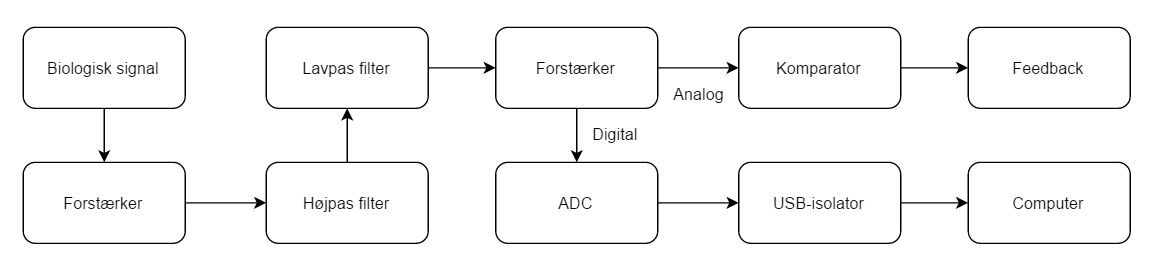
\includegraphics[scale=0.7]{figures/cProblemloesning/Systemopbygning.PNG}
	\caption{Figuren viser de enkelte blokke, som systemet skal indeholde.}
	\label{kravblok}
\end{figure}

Signalerne fra accelerometeret skal forstrækes, herefter støj skal filteres fra for at dæmpe uønskede frekvenser. Herefter forstærkes signalet med en variabel forstærkningen, da signalet kun er forstærket lidt. Signalet forstærkes til maksimalt 3V. Dette gøres ved en operationsforstærker \fxnote{inverteret eller ikke-inverteret} Det analoge signal ensrettet via. \fxnote{helbølgeensretter eller halvbølgeensretter}, hvor efter der benyttes en integrator til at lave en lineær linje. Ud fra denne linje gives en advarsel via feedback. Det digitale signal skal konverteres fra analogt til digitalt, hvilket gøres ved en ADC.  Herefter anvendes en USB-isolator for patientsikkerhed. Computeren skal fremvise en graf når NIDAQ er tilsluttet. 

\subsection{Kravspecifikationer}
For at gøre anvendelse af samme system muligt til 4. Semester skal arbejdsområdet kunne benyttes sammen med et USB-baseret trådløst udviklingsværktøj eZ430-RF2500 fra Texas Instruments. Det er derfor nødvendigt, at designet stemmer overens med udviklingsværktøjet for at kunne sende og modtage data til og fra computeren. Udviklingsværktøjet indeholder hardware og software som evaluerer mikrokontrolleren MSP430F2274. For at hele vores system kan anvendes med udviklingsværktøjet, skal outputsignalet være 0-3V, eftersom mikrokontrolleren opererer med spændingsforsyning mellem 1,8V og 3,6V. \\
I praksis er det ikke muligt at have ideelle komponenter. Der vurderes derfor ud fra et pilotforsøg den tolerance, der accepteres ift. de enkelte blokke i systemet. Dette er udført mhp. at kunne beregne forstærkning, filtrering og integrering af signalet.\fxnote{Husk at opdatere her, når der kommer flere blokke}

\subsubsection{Det samlede system}
Aktivering af bestemte dioder skal afspejle inputsignalet således at et lille input aktiverer en gul diode og vibration, mens et større input aktiverer en rød diode og stigningen i vibration. \fxnote{Evt. omformuler og skrive mere til}

\textbf{Overordnede krav til systemet:}
\begin{itemize}
\item Grøn diode: Skal lyse, når patienten ikke er ude i risikozonerne.  
\item Gul diode: Skal lyse, når patienten hælder 5$^{\circ}$ og slukke, hvis patienten retter sig op eller hælder yderligere.
\item Rød diode: Skal lyse, når patienten hælder 10$^{\circ}$ eller mere og slukke, hvis patienten retter sig op.
\item Vibration: Skal aktiveres, hvis patienten hælder 5$^{\circ}$ og skal slukke, hvis patienten retter sig op. Hvis patienten hælder yderligere, skal vibrationen stige.
\item Der skal være en sammenhæng mellem inputsignalets størrelse og antallet af dioder der lyser.
\item Signalet i systemet må ikke forstærkes til en værdi over 3V.
\end{itemize}



%\textbf{Tolerance:}
%\begin{itemize}
%\end{itemize}
%
%\subsubsection{Accelerometer}
%\textbf{Krav:}
%\begin{itemize}
%\end{itemize}
%
%\textbf{Tolerance:}
%\begin{itemize}
%end{itemize}
%
%\subsubsection{Instrumentering forstærker}
%\textbf{Krav:}
%\begin{itemize}
%\end{itemize}
%
%\textbf{Tolerance:}
%\begin{itemize}
%\end{itemize}
%
%\subsubsection{Filtre - opdeling i høj og lavpass?}
%\textbf{Krav:}
%\begin{itemize}
%\end{itemize}
%
%\textbf{Tolerance:}
%\begin{itemize}
%\end{itemize}

%\subsubsection{Forstærker med variabel forstærkning}

%\textbf{Krav:}
%\begin{itemize}
%\end{itemize}
%
%\textbf{Tolerance:}
%\begin{itemize}
%\end{itemize}
%
%\subsubsection{Ensretter}

%\textbf{Krav:}
%\begin{itemize}
%\end{itemize}
%
%\textbf{Tolerance:}
%begin{itemize}
%end{itemize}
%
%\subsubsection{Integrator}
%\textbf{Krav:}
%\begin{itemize}
%\end{itemize}
%
%\textbf{Tolerance:}
%\begin{itemize}
%\end{itemize}
%
%\subsubsection{Advarsel}
%\textbf{Krav:}
%\begin{itemize}
%\end{itemize}
%
%\textbf{Tolerance:}
%\begin{itemize}
%\end{itemize}
%
%\subsubsection{ADC}
%\textbf{Krav:}
%\begin{itemize}
%\end{itemize}
%
%\textbf{Tolerance:}
%\begin{itemize}
%\end{itemize}
%
%\subsubsection{USB-isolator}
%\textbf{Krav:}
%\begin{itemize}
%\end{itemize}
%
%\textbf{Tolerance:}
%\begin{itemize}
%\end{itemize}
%
%\subsubsection{Computer}
%\textbf{Krav:}
%\begin{itemize}
%\end{itemize}
%
%\textbf{Tolerance:}
%\begin{itemize}
%\end{itemize}
%\begin{itemize}
%\item Systemet skal ved fald få dioder til at lyse samt give feedback i form af stigende vibration. 
%\item Systemet skal være non-invasiv - dvs. systemet ikke må påføre patienten smerte eller varig skade
%\item Systemet skal være brugervenligt
%\item Systemet skal forsynes med spænding fra 9V batteri
%\end{itemize}

%\subsubsection{Accelerometer}
%Accelerometeret skal detektere patientens kropshældning.

%\subsubsection{Filter}
%Når der anvendes et filter, skal det dæmpe uønskede frekvenser. Dvs. frekvenser der lavere eller højere ift. det signal fra accelerometeret, som man vil analysere på. Der skal udføres et pilotforsøg for at finde frem til det korrekte filter og valg af knækfrekvens. 

%\subsubsection{Signalerende lys}
%Når patienten er ude af balance skal en rød diode lyse, som signalering ift. patientens hældning. Der skal vha. et pilotforsøg detekteres, hvornår dioden skal lyse. Skal der evt. være 2 dioder, hvor den ene er et "advarende" signal og nr. to er "fare". 

%\subsubsection{Alarm/vibrationen}
%Alarmen/vibrationen skal anvendes i perioden, hvor patienten er ude af balance og stoppe igen, når der igen er oprettet balance. 
%(eller fungere som en alarm til dioderne - så når en diode lyser, skal alarmen gå)

%\subsubsection{ADC}
%Der anvendes en ADC i systemet, for at konvertere det analoge signal til digitalt. Det næste skridt er konverteringen til PC og det er derfor essentielt at have en ADC, der konverterer analogt signal til binære tal, som digitale systemet anvender. 
%{Her skal vi have valgt en samplingsfrekvens)

%\subsubsection{USB-isolater}
%USB-isolatoren sikre patientens sikkerhed. Her skal input- og outputspænding være ens.  

%\subsubsection{Til PC}
%Fremvisning af graf, så patienten og plejepersonale kan følge %rehabiliteringens udvikling. 
